%!TEX root = ../masters_thesis.tex

\section{Editing Hivent Data} % (fold)
\label{sec:editing_hivent_data}

The previous section proposed the abstract Hivent Model, a set of Hivent Operations and the HistoGraph visualization. However, one purpose of the HGIS developed in this thesis is to add, alter and delete historical changes. This section presents the tools and methods to edit spatio-temporal data about the history of Areas in the Hivent Model. Whereas the Hivent Operations are well-defined and specific, user studies have shown that they are not well understood by humans for edit purposes. This chapter introduces a different set of six \emph{Edit Operations} in section \ref{sub:edit_operations}. Afterwards, section \ref{sub:edit_workflow} shows a \emph{workflow} to perform an Edit Operation step by step. The Hivent Model needs to support editing historical changes in between other historical changes. The last section \ref{sub:retrospective_updates} explains the theoretical approach to \emph{retrospecitve updates} of spatio-temporal data in the Hivent Model.

% ------------------------------------------------------------------------------
\subsection{Edit Operations} % (fold)
\label{sub:edit_operations}

The Hivent Operations are valuable, because they can describe all possible changes in the development of Areas in time and space. They are well understood by the system and form the basis for the Hivent Model. However, interviews with researchers in humanities at University of Virginia were conducted to understand their mental model about editing the history of countries on the map. It turned out that the Hivent Operations are not suitable for a human, because of their low-level nature. One example is that the operations do not provide a simple way to create a new Area on previously unclaimed land. Changing the formal name of an Area with a \texttt{UNI} operation is also not intuitive. Since a main goal of this thesis is to develop a user interface that humans can understand, a second set of six high-level \emph{Edit Operations} is proposed. They are shown in table \ref{tab:edit_operations}.

\vspace{0.5em}
\begin{table}[H]
\begin{center}
\begin{tabular}{m{0.75cm} m{0.8cm} m{2.4cm} m{9.1cm}}
  \toprule

  \raisebox{-0.35\height}
  {
\includegraphics[width=0.72cm]{graphics/development/editing_hivent_data/edit_operations/CRE}} &
  \texttt{CRE} & Create &
  a new Area with a new name and territory on the map. \\

  \midrule
  \raisebox{-0.35\height}
  {
\includegraphics[width=0.72cm]{graphics/development/editing_hivent_data/edit_operations/MRG}} &
  \texttt{MRG} & Merge &
  two or more Areas to a new Area. The name has to be set manually, the territory is automatically unified. \\

  \midrule
  \raisebox{-0.35\height}
  {
\includegraphics[width=0.72cm]{graphics/development/editing_hivent_data/edit_operations/DIS}} &
  \texttt{DIS} & Dissolve &
  one Area into two or more new Areas, manually setting their new territory and name. \\

  \midrule
  \raisebox{-0.35\height}
  {
\includegraphics[width=0.72cm]{graphics/development/editing_hivent_data/edit_operations/CHB}} &
  \texttt{CHB} & Change Borders &
  between two neighboring Areas by defining the territory that changes sides. \\

  \midrule
  \raisebox{-0.35\height}
  {
\includegraphics[width=0.72cm]{graphics/development/editing_hivent_data/edit_operations/REN}} &
  \texttt{REN} & Rename &
  an Area and set a new formal name, short name or both. \\

  \midrule
  \vspace{0.35em}
  \raisebox{-0.35\height}
  {
\includegraphics[width=0.72cm]{graphics/development/editing_hivent_data/edit_operations/CES}} &
  \texttt{CES} & Cease &
  an Area by deleting it from the map, leaving unclaimed land. \\

  \bottomrule
\end{tabular}
\caption{The six Edit Operations}
\label{tab:edit_operations}
\end{center}
\end{table}

% - - - - - - - - - - - - - - - - - - - - - - - - - - - - - - - - - - - - - - -
\paragraph{Error correction} % (fold)
\label{par:error_correction}

Another use case for the interface is to correct wrong information on the map. For this purpose it is important to understand how correcting information in an event-based system works: Given an Area $A$ at time point $t_y$. The name of $A$ at this point should be $Y$, but happens to be $X$. That means the operation at $t_x: t_x < t_y$ that created the name $X$ for Area $A$ is erroneous and has be corrected. Correcting a state means correcting the operation that created this state.

% paragraph error_correction (end)

% subsection edit_operations (end)

% ------------------------------------------------------------------------------
\subsection{Edit Workflow} % (fold)
\label{sub:edit_workflow}

The Edit Operatoins have proven to be understandable in several user studies. This section shows they can be internally expressed by a set of Hivent Operations. The creation of an Edit Operation happens in four steps of a simple workflow:

\begin{compactenum}
  \item Select the Areas that will be changed in the operation.
  \item For each new Area resulting from the operation, create a territory.
  \item For each new Area create a name.
  \item Add the Edit Operation to an Hivent to inherit the time point.
\end{compactenum}

For each Edit Operation the requirements for the steps are different. Not all operations need all steps, since some data can be processed automatically. Table \ref{tab:editoperations_in_worklow} presents an overview about the behavior of the Edit Operations in the first three steps. The last step is necessary for each operation alike.


\vspace{1em}
\begin{table}[H]
\begin{center}
\begin{tabular}{m{0.9cm} m{4.2cm} m{4.2cm} m{3.5cm}}
  \toprule

  &
  \emph{Select old Areas} &
  \emph{Create new territories} &
  \emph{Create new names} \\

  \midrule
  \texttt{CRE} &
  -- &
  create a territory of the new country &
  create a name for the new country \\

  \midrule
  \texttt{MRG} &
  select the countries to be merged &
  \pbox{4.4cm}{--\\
  \footnotesize{\emph{territories of selected countries are automatically unified}}} &
  create a name for the new country
  \\

  \midrule
  \texttt{DIS} &
  select a country to be \mbox{dissolved} &
  create a territory for each new country &
  create a name for each new country \\

  \midrule
  \texttt{CHB} &
  select two neighboring countries to change their border &
  \pbox{4.4cm}{create the new border between both countries \\
  \footnotesize{\emph{the territory for both countries will be created automatically}}}  &
  -- \\

  \midrule
  \texttt{REN} &
  select a country to rename it &
  -- &
  create a new name of the country \\

  \midrule
  \texttt{CES} &
  select a country to cease it &
  -- &
  -- \\

  \bottomrule
\end{tabular}
\caption{The requirements of each step for the Edit Operations}
\label{tab:editoperations_in_worklow}
\end{center}
\end{table}

% - - - - - - - - - - - - - - - - - - - - - - - - - - - - - - - - - - - - - - -

% wording:
% UNI of "[old]"  to    "new"
% INC of "[old]"  into  "pres"
% SEP of "old"    into  "[new]"
% SEC of "[new]"  from  "pres"
% NCH of "pres"

\vspace{-1.0em}

Depending on the input of the user in the steps for an Edit Operation, there are different possibilities to express it by a set of Hivent Operations. All possibilities are introduced in table \ref{tab:editoperations_to_hg_operations}. Hivent Operations are combined when they happen at the same time. In the example of the German Reunification, East Germany was incorporated into West Germany which at the same time changed its short name to ``Germany'' (\texttt{INC + NCH}).

\begin{center}
\begin{longtable}{m{1.2cm} m{0.95cm} m{0.95cm} m{0.95cm} m{6.0cm} m{2.3cm}}
  \toprule

  \pbox{1.2cm}{EditOp.\\(case)} &
  \pbox{0.95cm}{old\\Areas\\[-0.8em]} &
  \pbox{0.95cm}{update\\Areas\\[-0.8em]} &
  \pbox{0.95cm}{new\\Areas\\[-0.8em]} &
  expression by Hivent Operations &
  visualization \\
  \midrule
  \endhead

  % TODO: introduce T as territory that is used like a temporary Area with exactly that territoy

  %%% CREATE %%

  \multirow{9}{*}{\texttt{CRE} (1)} &
  \multicolumn{4}{p{10cm}}{
    The Area $B_1$ is created with territory $T$. The part of $T$ that is on previously unclaimed land ($T_\Omega$) is seceded as $B_1$ from $\Omega$.
    If $T_\Omega$ is empty, then $B_1$ is initialized with an empty territory.
    The rest of $T$ covers some Areas $P_i \in P$ partially and some Areas $F_i \in F$ fully.
    $\forall P_i:$ the covered territory $T_i$ is seceded and incorporated into $B_1$.
    $\forall F_i: F_i$ is completely incorporated into $B_1$.
  } &
  \multirow{9}{*}{
    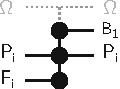
\includegraphics[width=2.5cm]{graphics/development/editing_hivent_data/edit_to_hivent_operations/CRE_to_SEC+UNI}
  } \\

  &
  $\forall F_i$ &
  $\forall P_i$ &
  $B_1$ &
  \pbox{6.0cm}{
    ~\\
    \texttt{SEC} of $B_1$ from $\Omega$ \\
    \texttt{SEC} of $T_i$ from $P_i$, \texttt{INC} of $T_i$ into $B_1$ \\
    \texttt{INC} of $F_i$ into $B_1$
  } &
  \\

  %%% MERGE %%

  \midrule
  \multirow{3}{*}{\texttt{MRG} (1)} &
  \multicolumn{4}{p{10cm}}{
    Multiple Areas $A_i \in A, |A| \geq 2$ are unified to $B_1$. The new Area receives a name distinct from all the names of $A_i$.
  } &
  \multirow{3}{*}{
    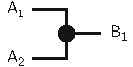
\includegraphics[width=2.5cm]{graphics/development/editing_hivent_data/edit_to_hivent_operations/MRG_to_UNI}
  } \\
  &
  $\forall A_i$ &
  -- &
  $B_1$ &
  \pbox{6.0cm}{
    \texttt{UNI} of $\forall A_i$ to $B_1$
  } &
  \\

  \midrule
  \multirow{4}{*}{\texttt{MRG} (2)} &
  \multicolumn{4}{p{10cm}}{
    Multiple Areas $A_i \in A, |A| \geq 2$ are unified. The resulting Area reuses the short and formal name of one of the old Areas ($A_0$) and therefore preserves it. The remaining Areas $A_i$ are incorporated into $A_0$.
  } &
  \multirow{4}{*}{
    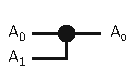
\includegraphics[width=2.5cm]{graphics/development/editing_hivent_data/edit_to_hivent_operations/MRG_to_INC}
  } \\
  &
  $\forall A_i$ &
  $A_0$ &
  -- &
  \pbox{6.0cm}{
    \texttt{INC} of $\forall A_i$ into $A_0$
  } &
  \\

  \midrule
  \multirow{4}{*}{\texttt{MRG} (3)} &
  \multicolumn{4}{p{10cm}}{
    The same as the previous case, just that $A_0$ receives a new short name and therefore an additional name change is required.
  } &
  \multirow{4}{*}{
    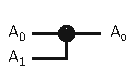
\includegraphics[width=2.5cm]{graphics/development/editing_hivent_data/edit_to_hivent_operations/MRG_to_INC+NCH}
  } \\
  &
  $\forall A_i$ &
  $A_o$ &
  -- &
  \pbox{6.0cm}{
    ~\\
    \texttt{INC} of $\forall A_i$ into $A_0$ \\
    \texttt{NCH} of $A_0$
  } &
  \\

  %%% DISSOLVE %%

  \midrule
  \multirow{4}{*}{\texttt{DIS} (1)} &
  \multicolumn{4}{p{10cm}}{
    Multiple Areas $B_i$ are separated from one initial Area $A_1$. Each $B_i$ receives a part of the territory of $A_1$ and a name. Each name is distinct from the name of $A_1$.
  } &
  \multirow{4}{*}{
    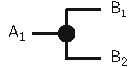
\includegraphics[width=2.5cm]{graphics/development/editing_hivent_data/edit_to_hivent_operations/DIS_to_SEP}
  } \\
  &
  $A_1$ &
  -- &
  $\forall B_i$ &
  \pbox{6.0cm}{
    ~\\
    \texttt{SEP} of $A_1$ into $\forall B_i$
  } &
  \\

  \midrule
  \multirow{5}{*}{\texttt{DIS} (2)} &
  \multicolumn{4}{p{10cm}}{
    Multiple Areas $B_i$ are separated from one initial Area $A_0$. Each $B_i$ receives a part of the territory of $A_0$ and a name. One of the separated Areas has the same short and formal name as $A_0$, so it preserves its identity. The remaining new Areas secede from $A_0$.
  } &
  \multirow{5}{*}{
    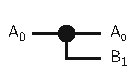
\includegraphics[width=2.5cm]{graphics/development/editing_hivent_data/edit_to_hivent_operations/DIS_to_SEC}
  } \\
  &
  -- &
  $A_0$ &
  $\forall B_i$ &
  \pbox{6.0cm}{
    ~\\
    \texttt{SEC} of $\forall B_i$ from $A_0$
  } &
  \\

  \midrule
  \multirow{4}{*}{\texttt{DIS} (3)} &
  \multicolumn{4}{p{10cm}}{
    The same as the previous case, just that $A_0$ receives a new short name and therefore an additional name change is required.
  } &
  \multirow{4}{*}{
    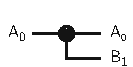
\includegraphics[width=2.5cm]{graphics/development/editing_hivent_data/edit_to_hivent_operations/DIS_to_SEC+NCH}
  } \\
  &
  -- &
  $A_0$ &
  $\forall B_i$ &
  \pbox{6.0cm}{
    ~\\
    \texttt{SEC} of $\forall B_i$ from $A_0$  \\
    \texttt{NCH} of $A_0$
  } &
  \\

  %%% CHANGE BORDER %%%

  \midrule
  \multirow{10}{*}{\texttt{CHB} (1)} &
  \multicolumn{4}{p{10cm}}{
    One existing Area $A_0$ is selected and its territory changes. Relative to the old territory some parts of the territory expands ($T_e$) and some withdraws ($T_w$).
    The part of $T_e$ that expands into unclaimed land ($T_\Omega: T_\Omega \in T_e$) is seceded from $\Omega$ and incorporated into $A_0$.
    The Areas $F_i$ fully covered by $T_e$ are incorporated into $A_0$,
    the Areas $P_i$ partially covered by $T_e$ secede this territory $T_i \in T_e$ to $A_0$.
    $T_w$ is be incorporated into $\Omega$, resulting in unclaimed land.
  } &
  \multirow{10}{*}{
    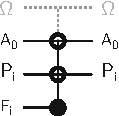
\includegraphics[width=2.5cm]{graphics/development/editing_hivent_data/edit_to_hivent_operations/CHB_to_SEC+INC_omega}
  } \\
  &
  $\forall F_i$ &
  $A_0, \forall P_i$ &
  -- &
  \pbox{6.0cm}{
    ~\\
    \texttt{SEC} of $T_\Omega$ from $\Omega$,
    \texttt{INC} of $T_\Omega$ into $A_0$ \\
    \texttt{SEC} of $T_i$ from $P_i$,
    \texttt{INC} of $T_i$ into $B_1$ \\
    \texttt{INC} of $F_i$ into $B_1$ \\
    \texttt{SEC} of $T_w$ from $B_1$,
    \texttt{INC} of $T_w$ into $\Omega$
  } &
  \\

  \midrule
  \multirow{7}{*}{\texttt{CHB} (2)} &
  \multicolumn{4}{p{10cm}}{
    Two existing Areas $A_1$ and $A_2$ are selected and their common border changes. This results in a symmetrical change of territories, made up by two sets of territories: $T_2$ that previously belonged to $A_1$ and is now part of $A_2$ and $T_1$ for which the opposite is true. $T_2$ is seceded by $A_1$ and incorporated into $A_2$, the opposite happenes to $T_1$.
  } &
  \multirow{7}{*}{
    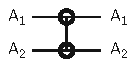
\includegraphics[width=2.5cm]{graphics/development/editing_hivent_data/edit_to_hivent_operations/CHB_to_SEC+INC}
  } \\
  &
  -- &
  $A_1, A_2$ &
  -- &
  \pbox{6.0cm}{
    ~\\
    \texttt{SEC} of $T_2$ from $A_1$,
    \texttt{INC} of $T_2$ into $A_2$ \\
    \texttt{SEC} of $T_1$ from $A_2$,
    \texttt{INC} of $T_1$ into $A_1$
  } &
  \\

  %%% RENAME %%%

  \midrule
  \multirow{3}{*}{\texttt{REN} (1)} &
  \multicolumn{4}{p{10cm}}{
    One Area $A_1$ is selected and both its short and formal name is changed. Therefore, a new Area $B_1$ is created as a direct successor of $A_1$. This is a special case of a unification with only one Area.
  } &
  \multirow{3}{*}{
    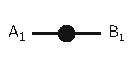
\includegraphics[width=2.5cm]{graphics/development/editing_hivent_data/edit_to_hivent_operations/REN_to_UNI}
  } \\
  &
  $A_1$ &
  -- &
  $B_1$ &
  \pbox{6.0cm}{
    \texttt{UNI} of $A_1$ to $B_1$
  } &
  \\

  \midrule
  \multirow{3}{*}{\texttt{REN} (2)} &
  \multicolumn{4}{p{10cm}}{
    One Area $A_1$ is selected and receives a new short name, but the formal name and therefore the identity is preserved. $A_1$ is updated.
  } &
  \multirow{3}{*}{
    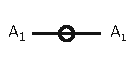
\includegraphics[width=2.5cm]{graphics/development/editing_hivent_data/edit_to_hivent_operations/REN_to_NCH}
  } \\
  &
  -- &
  $A_1$ &
  -- &
  \pbox{6.0cm}{
    \texttt{NCH} of $A_1$
  } &
  \\

  %%% CEASE %%%

  \midrule
  \multirow{2}{*}{\texttt{CES} (1)} &
  \multicolumn{4}{p{10cm}}{
    One Area $A_1$ is selected and ceases by incorporating into the universe.
  } &
  \multirow{2}{*}{
    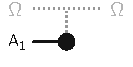
\includegraphics[width=2.5cm]{graphics/development/editing_hivent_data/edit_to_hivent_operations/CES_to_INC}
  } \\
  &
  $A_1$ &
  -- &
  -- &
  \pbox{6.0cm}{
    \texttt{INC} of $A_1$ into $\Omega$
  } &
  \\

  \bottomrule
\caption{Translation from Edit Operations to Hivent Operations.\protect\footnotemark}
\end{longtable}
\label{tab:editoperations_to_hg_operations}
\end{center}

\footnotetext{multiple Hivent Operations in one row happen exactly at the same time point, so they are combined}

% subsection edit_workflow (end)

% ------------------------------------------------------------------------------
\subsection{Retrospective Updates} % (fold)
\label{sub:retrospective_updates}

A straightforward use case of the Hivent Model is to change the current state of the system with a new Hivent Operation into the future. Givent the initial start point $t_0$, a current time point $t_{now} > t_0$ and a set of consecutively added Hivent Operations at $\forall t_i: t_0 \leq t_i < t_{now}$. The accumulation of all changes make up the current state of the system at $t_{now}$. To change this current state, a new Hivent Operation can be inserted at $t_{now}$ into the future. This state is valid until the next change is inserted.

For historical research that use case alone is not sufficient, because the current state of the map at $t_{now}$ (2016) is known to a large degree. The problem is to describe states and changes in the past. Therefore the systems needs to support entering Hivent Operations in between other existing operations.


% - - - - - - - - - - - - - - - - - - - - - - - - - - - - - - - - - - - - - - -
\paragraph{Integrity} % (fold)
\label{par:integrity}

Each Hivent Operation that is not entered to the end of the timeline must maintain the semantic, spatial and thematic integrity of the data, i.e. the changes to Areas, their territories and names must still work. The simple example in figure \ref{fig:update_conflict_example} shows the problem: Given time point $t_1$ with two Areas $A$ and $B$ and an \texttt{UNI} Hivent Operation at $t_2$ unifying $A$ and $B$ to $C$. If in retrospective a new Hivent Operation is inserted at $t_r: t_1 < t_r < t_2$ that cedes a part of of $A$ to a new Area $X$, the operation at $t_2$ is not consistent anymore, because the old territory of $A$ is not the same. It is not simple to say how the remaining territory $?$ should be treated.

\begin{figure}[H]
  \vspace{1em}
  \centering
  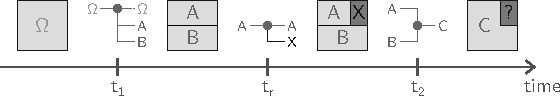
\includegraphics[width=0.8\textwidth]{graphics/development/editing_hivent_data/retrospective_updates/example}
  \caption{Example for a simple conflict due to a retrospective update}
  \label{fig:update_conflict_example}
\end{figure}

% paragraph integrity (end)

% - - - - - - - - - - - - - - - - - - - - - - - - - - - - - - - - - - - - - - -
\paragraph{Conflicts} % (fold)
\label{par:conflicts}

The way the Hivent Model works is comparable to a version control system like \emph{Git}
\footnote{
  \emph{Git},
  - -everything-is-local,
  \url{https://git-scm.com/},
  last access: 29.05.2016
}
There are different kinds of conflicts that can occur on retrospective updates. In the Hivent Model, they are classified regarding their resolvability:

\begin{compactenum}
  \item[A)] The conflict can be resolved \emph{\textbf{a}utomatically} without the interference of the user.
  \item[S)] The conflict requires the user to choose between two alternatives (\emph{\textbf{s}emi-automatic} resolution).
  \item[M)] The conflict is complex and the user needs to resolve it \emph{\textbf{m}anually}.
\end{compactenum}

The remaining part of this section examines all possible cases of conflicts and their resolveability. Each inserted Hivent Operation transforms a set of old Areas $A = [A_i]$ to a set of new Areas $B = [B_i]$ or updates an update Area $A_0$ or both. Each consecutive Hivent Operation that manipulates $A_0, A_i \in A$ or $B_i \in B$ has to be checked regarding three aspects of integrity:

\begin{compactenum}
  \item semantic: Does $A_0$ and $\forall A_i \in A$ still exist? If not, can it easily be replaced by another Area?
  \item spatial: Is the territory of $A_0$ and $\forall A_i \in A$ still the same? If not, can it easily by updated?
  \item thematic: Is the name of $A_0$ and $\forall A_i \in A$ still the same? If not, can it easily be updated?
\end{compactenum}

All cases can be simulated in the following simple scenario: Given the system with only two states: an initial state at $t_1$ at which only three spatial entities are on the map ($A_1, A_2, A_3$) and an Hivent Operation at $t_2$ that manipulates some of these Areas with one of the five possible operations. This is called the original Hivent Operation ($H_o$). Now, a retrospective update $H_r$ is inserted in between the two states ($t_r: t_1 < t_r < t_2$). $H_r$ manipulates the same set of Areas with an Hivent Operations. The question is: What happens regarding the semantic, spatial and thematic integrity of $H_o$? Is there a conflict and if so, hw can it be resolved? There are 25 possible cases, because for both $H_o$ and $H_r$ there are five possible Hivent Operations.

% paragraph conflicts (end)

% - - - - - - - - - - - - - - - - - - - - - - - - - - - - - - - - - - - - - - -
\paragraph{Retrospective Name Change} % (fold)
\label{par:retrospective_name_change}

The first five cases are straightforward: Given \texttt{NCH} is inserted in retrospective ($H_r$) to change the name of $A_1$ from $X$ to $Y$. This has no effect on the identity or territory of $A_1$. Therefore the system only needs to check for thematic integrity of $H_o$. If that operation is an \texttt{INC} or \texttt{SEC}, which both only change the territory of $A_1$, it is not conflicting. If $H_o$ is a \texttt{UNI} or \texttt{SEP}, then there is a conflict: $A_1$ is an old Area of the operation, but the name associated to $A_1$ is still $X$. This is not consistent, because $H_r$ just changed the name to $Y$ . This conflict can be resolved automatically by updating the name in the old Area from $X$ to $Y$. The same is true if $H_o$ is a \texttt{NCH} operation: $A_1$ is the update Area and the old name has to be updated from $X$ to $Y$. To summarize what the system has to do if a \texttt{NCH} on $A_1$ is inserted in retrospective: find the next \texttt{UNI}, \texttt{SEP} or \texttt{NCH} operation that manipulates $A_1$ and update its old name.

% paragraph retrospective_name_change (end)

% - - - - - - - - - - - - - - - - - - - - - - - - - - - - - - - - - - - - - - -
\paragraph{Retrospective Incorporation} % (fold)
\label{par:retrospective_incorporation}

An \texttt{INC} ceases a set of old Areas and changes the territory of one Area. In this scenario, $H_r$ incorporates $A_2$ into $A_1$. The question is what kind of conflicts can occur to the spatial integrity of $H_o$? If $H_o$ is  a \texttt{NCH}, there is no conflict, because $H_o$ changes the territory of $A_1$ and \texttt{NCH} the name.

\begin{figure}[ht]
\vspace{1em}
  \centering
  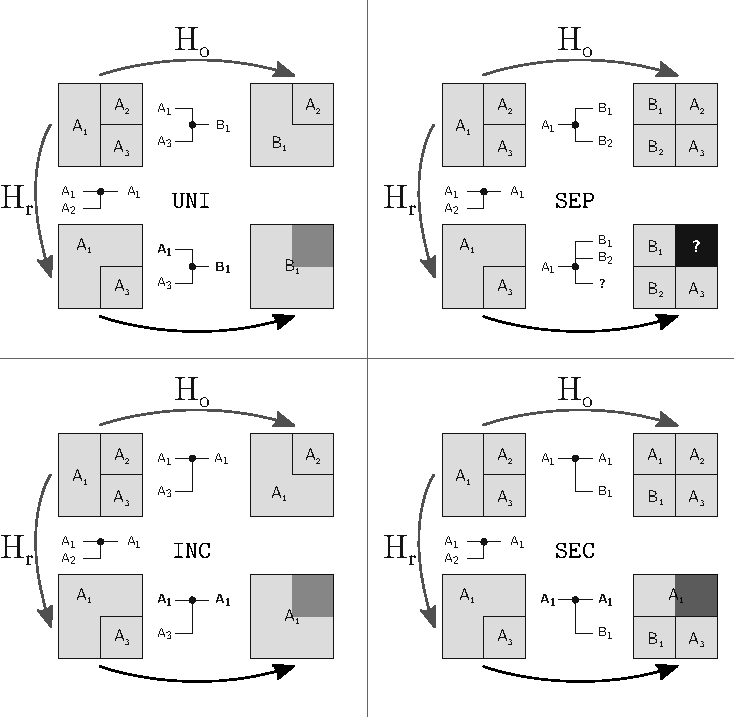
\includegraphics[width=0.8\textwidth]{graphics/development/editing_hivent_data/retrospective_updates/INC}
  \caption{Conflicts after a retrospective incorporation}
  \label{fig:update_conflict_INC}
\end{figure}

Figure \ref{fig:update_conflict_INC} shows the conflicts that occur in the remaining four possiblities of $H_o$. In the case of an original \texttt{UNI} operation, it can still be performed with the same Areas, because $H_r$ did not change the identity of $A_1$. However, the territory of $A_1$ has been enlarged. This new territory has to be taken into account for $H_o$: To maintain spatial integrity, the system has to update the territory of incoming $A_1$. However, the territory of $B_1$ has to be updated as well, because it is enlarged in the same way as $A_1$. This requires a recursive update into the future: the next Hivent Operation dealing with $B_1$ needs to take into account that the territory has changed. This case can be treated as if $H_o$ would be $H_r$ with an \texttt{INC} operation. The system has to repeat this process until all conflicts are solved. The same is true if $H_o$ is an \texttt{INC} operation: The system needs to update the old and the new territory of $A_1$ in $H_o$ and recursively update the territory of $A_1$ into the future.

If $H_o$ is a \texttt{SEP} operation, there is a major conflict: originally, $A_1$ splitted into $B_1$ and $B_2$. Due to $H_r$, the territory of $A_1$ is larger. $H_o$ can still separate $B_1$ and $B_2$ from $A_1$ the same way as before, but it is unclear what should happen to the remaning territory of $A_1$ that has just been enlarged. This conflict has to be resolved manually, because the system can not derive a decision from any existing information. The remaining part could become $\Omega$, it could be incorporated into $B_1$ or $B_2$ or stay $A_1$. However, the user has to decide it. In case of an original \texttt{SEC}, the situation is slightly different: $H_1$ still exists like before, just with a larger territory. $H_o$ can secede $B_1$ like originally, but the system needs to update the old and new territory of $A_1$ in this operation and recursively into the future.

The foregoing investigation relates only to $A_1$ but not to $A_2$ that has been incorporated into $H_r$. From the perspective of $A_2$, this change can be seen as a \texttt{UNI}, because its identity ceases and together with its territory it completely merges into $A_1$. Therefore this is treated like a retrospective unification examined later in this section.

% paragraph retrospective_incorporation (end)

% - - - - - - - - - - - - - - - - - - - - - - - - - - - - - - - - - - - - - - -
\paragraph{Retrospective Secession} % (fold)
\label{par:retrospective_secession}

Retrospective secessions are comparable to incorporations: The identity and the name of $A_1$ does not change -- but parts of its territory ceases to a new Area $B_1$. This section examines how the system has to treat $B_1$ and the smaller territory of $A_1$ in the original operation $H_o$. Exactly like for retrospective incorporation, there is no conflict if $H_o$ is a \texttt{NCH}.

\begin{figure}[ht]
\vspace{1em}
  \centering
  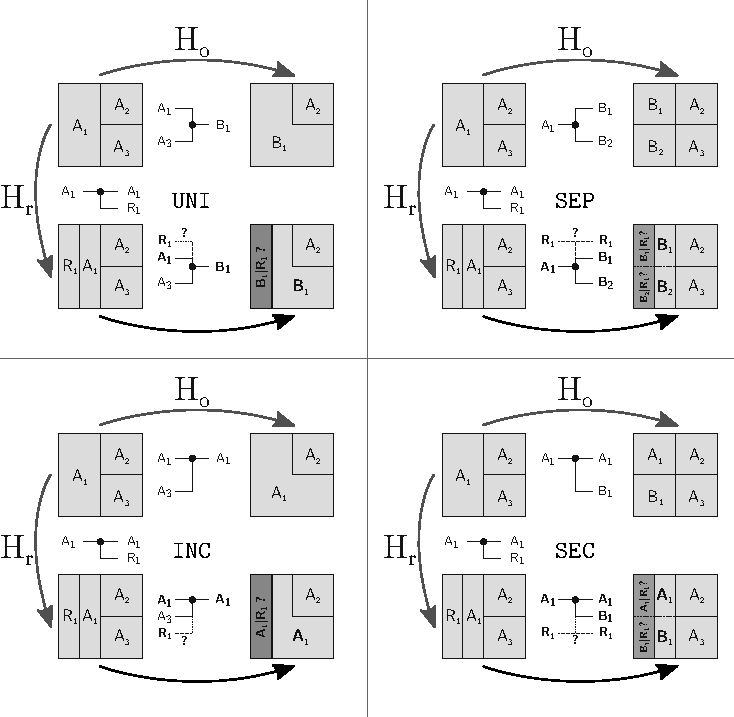
\includegraphics[width=0.8\textwidth]{graphics/development/editing_hivent_data/retrospective_updates/SEC}
  \caption{Conflicts after a retrospective secession}
  \label{fig:update_conflict_SEC}
\end{figure}

The other four cases are visualized in figure \ref{fig:update_conflict_SEC}. For an original \texttt{UNI}, there is a conflict: Originally, $A_1$ and $A_3$ unified to $B_1$. Although $H_r$ cedes parts of the territory of $A_1$ to $R_1$, $H_o$ can still merge it with $A_3$. The question is what happens to the remaining territory of $R_1$? There are two options:
\begin{compactenum}
  \item
  \emph{priority to $H_r$}:
  $R_1$ stays an own Area and is not affected by $H_o$.
  \item
  \emph{priority to $H_o$}:
  $H_o$ unifies $R_1$ to $B_1$ as well.
\end{compactenum}
For the system it is hard to decide this, because it is unclear what the intention of the user is when creating $R_1$ in $H_r$: Should the newly created Area be there for longer or is the territory of the unitied Area $A_3$ more important? In order for the system to not behave unexpectedly, it will ask the user which choice he or she prefers. In case of the first choice, the territory of $R_1$ has to be subtracted from the territory of the new Area $B_1$ in $H_o$. This update is again recursive, because the next Hivent Operation dealing with $B_1$ needs to operate on the correct territory as well. In the second case, $R_1$ simply has to be added to the old Areas of the \texttt{UNI} operation in $H_o$. No further recursive update is necessary. The same behavior is true if $H_o$ is an \texttt{INC}. The user has to decide if he or she wants to incorporate $R_1$ into $A_1$ or keep it as a separate Area. In the latter case, the system needs to update the new territory of $A_1$ in $H_o$.

For an original \texttt{SEP}, the situation is comparable: Originally, $A_1$ splits into $B_1$ and $B_2$, but after the restrospective secession of a part of $A_1$ to $R_1$, the territory of $R_1$ is conflicting with $B_1$ and $B_2$ in $H_o$. An important observation is that each part of $R_1$ would be part of either $B_1$ or $B_2$. There is no empty land, since both $R_1$ and $B_1+B_2$ seceded from the same territory of $A_1$. Just like the other two cases above, the system will give the user for both conflicting territories the choice if either $R_1$ should stay an Area or if $B_1$ respectively $B_2$ should incorporate $R_1$ into their territory. In the first case, the territory of $R_1$ has to be subtracted both from the incoming $A_1$ and recursively from the outgoing territory $B_1$ respectively $B_2$. The latter case needs at least one additional Hivent Operation: the part of $R_1$ that shall be part of $B_1$ respectively $B_2$ needs to be seceded from $R_1$ and the same time incorporated into $A_1$ which then again in the same moment is separated into $B_1$ and $B_2$ ($H_o$ = \texttt{SEC+INC+SEP}). If whole $R_1$ ceases in the operation, then it is incorporated into $A_1$ completely, so it is only a \texttt{INC+SEP} at $H_o$. The case of an orginal \texttt{SEC} the system behaves in exactly the same way, just with an update of the territory of $A_1$ and $B_1$ instead of $B_1$ and $B_2$.

To summarize, the main difference between retrospective incorporation and secession is that in the latter case, the user needs to choose between two predefined options. For incorporations, this is seen as unnecessary, because the conflicting territory of $A_2$ has not been manipulated by $H_o$, so it can not be seen as a concious decision of the user to keep this Area.

% paragraph retrospective_secession (end)

% - - - - - - - - - - - - - - - - - - - - - - - - - - - - - - - - - - - - - - -
\paragraph{Retrospective Unification} % (fold)
\label{par:retrospective_unification}

If a \texttt{UNI} is inserted in retrospective, the semantic integrity of $H_o$ is threatened, because in contrast to a \texttt{INC} all incoming Areas cease and unify to one completely new Area, in this example $R_1$. For each Area $A_i \in A$ that was unified in $H_r$ the system needs to find the next Hivent Operation $H_o$ manipulating $A_i$ and update it accordingly. In this example, $A_1$ is examined in place of each $A_i \in A$. If $H_o$ is a \texttt{NCH}, there is a conflict: the name of $A_1$ can obviously not be updated anymore, because $A$ does not exist aynmore. The only way to resolve this conflict is to automatically delete the \texttt{NCH} operation. All the other four cases behave regarding spatial integrity in exactly the same way as for a retrospective incorporation -- with the only difference that the Area $A_1$ is replaced by $R_1$ as an incoming Area in the operation. In all four cases, the territory has to be updated in the same way as for retrospective incorporation and the same conflict occurs for the original \texttt{SEP} operation.

\begin{figure}[ht]
\vspace{1em}
  \centering
  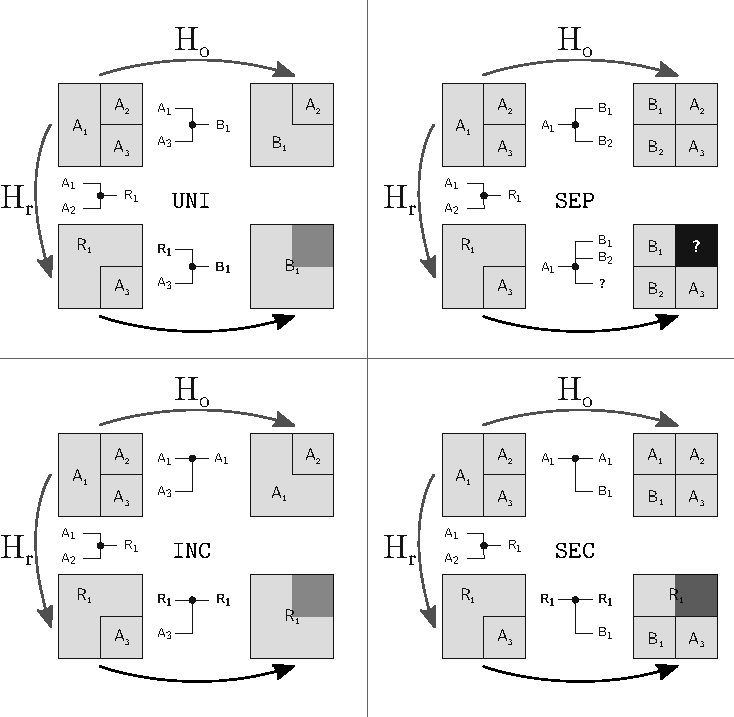
\includegraphics[width=0.8\textwidth]{graphics/development/editing_hivent_data/retrospective_updates/UNI}
  \caption{Conflicts after a retrospective unification}
  \label{fig:update_conflict_UNI}
\end{figure}

% paragraph retrospective_unification (end)

% - - - - - - - - - - - - - - - - - - - - - - - - - - - - - - - - - - - - - - -
\paragraph{Retrospective Separation} % (fold)
\label{par:retrospective_separation}

In contrast to the previous example, retrospective separations behave slightly different from secessions. $H_o$ has to be checked both for spatial and semantic integrity, since $A_1$ ceased in $H_r$ to a set of new Areas $R_i$. In this scenario, $R_1$ and $R_2$ stay in place for $\forall r_i \in R$. If $H_o$ is a \texttt{NCH}, the operation has to be automatically deleted, because $A_1$ does not exist anymore. Figure \ref{par:retrospective_separation} shows the conflicts that arise for the remaining four cases.

\begin{figure}[ht]
\vspace{1em}
  \centering
  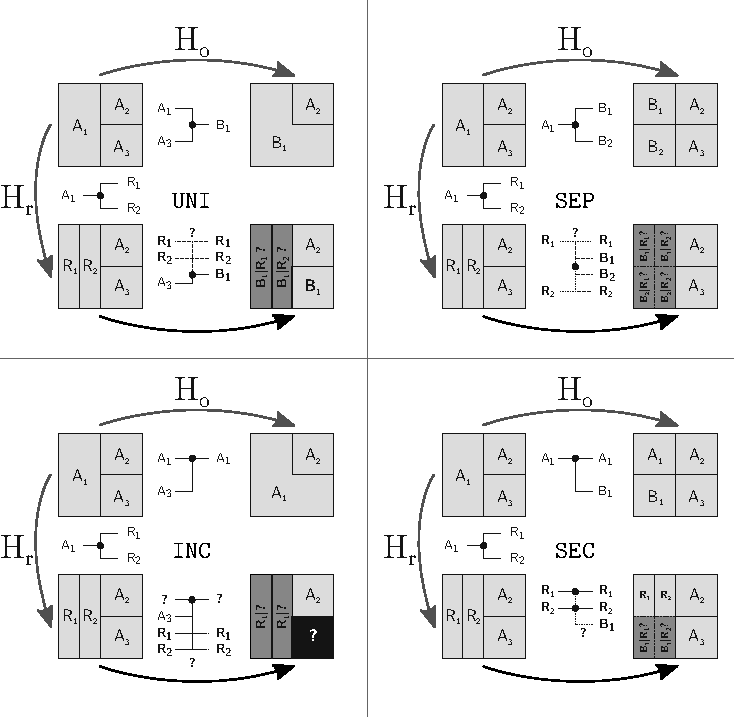
\includegraphics[width=0.8\textwidth]{graphics/development/editing_hivent_data/retrospective_updates/SEP}
  \caption{Conflicts after a retrospective separation}
  \label{fig:update_conflict_SEP}
\end{figure}

In case $H_o$ is a \texttt{UNI}, the arising conflict can be solved semi-automatically: originally, $B_1$ was created by unifying $A_1$ and $A_3$. $A_1$ just got separated into $R_1$ and $R_2$ by $H_r$, so the system can not know if $R_1$, $R_2$ or $B_1$ is preferred at $H_o$. In any case, the system needs to remove $A_1$ form the old Areas in the \texttt{UNI} operation. For each created Area in $H_r$ -- in this case only $R_1$ and $R_2$ -- the system asks the user if he or she prefers $R_i$ or $B_1$. If $R_1$ is preferred, then its territory has to be recursively subtracted from from the outgoing Area $B_1$ in the \texttt{UNI} operation at $H_o$. Else $R_i$ is added to the old Areas of $H_o$. If $R_i$ is preferred every time, the remaining \texttt{UNI} operation only transforms $A_3$ to $B_1$.

If $H_o$ is an \texttt{INC}, the situation is more complex: The Area $A_1$ in which $A_3$ should be incorporated into does not exist anymore. Moreover, it is replaced by a set of new Areas $R_i$ and it is not straightforward to see where $A_3$ should be incorporated into -- it is only clear that $A_3$ will cease in this operation. Since there is no information about what should be there instead, this conflict has be solved manually. The situation is even more complicated, because on the one hand, in $H_o$ the user intentionally incorporated $A_3$ into $A_1$ which means there is an obvious intention to keep $A_1$. On the other hand, he or she separated $A_1$ in $H_r$ to two new Areas $R_1$ and $R_2$, so also they can be seen as intenionally created. To avoid an unexpected behavior of the system, the best approach is give him or her the choice to keep $R_1$ and $R_2$, but in case of denial let the user resolve the whole conflict manually.

The case of an original \texttt{SEP} is likewise complex: $A_1$ does not exist anymore to be separated -- instead there are two sets of Areas that can be seen as reasonable to be the outcome of the operation: On the one hand the Areas $B_i \in B$ created in $H_o$ and on the other hand $R_j \in R$ created in $H_r$. Since it is impossible for the system to know which Areas to prefer, the user should decide for each possible combination $i \times j$ which Area it should be. If $R_j$ is preferred, then its territory has to be recursively subtracted from each $B_i$ that intersects with $R_j$. Else the territory of $R_j$ intersecting with $B_i$ has to secede from $R_j$ and be incorporated into $B_i$ with a combination of \texttt{SEC+INC} at $H_o$. The \texttt{SEP} operation itself it not necessary anymore, because there is not one simple old Area anymore.

The last case to examine is the influence of a retrospective \texttt{SEP} on an original \texttt{SEC}. Originally, $\forall B_i \in B$ would secede from $A_1$, which has just been separated into $\forall R_j \in R$ in $H_r$. The part of the territory of each $R_j \in R$ not covered by any $B_i \in B$ will certainly stay $R_j$, because there is no other reasonable alternative. The conflict is at the overlapping territory between $B_i$ and $R_j$. Just like for the previous example, the user has to resolve these conflicts semi-automatically by choosing either $B_i$ or $R_j$ for each possible alternative. If $B_i$ is preferred, it is seceded from the related $R_j$ at $H_o$. If $R_j$ is preferred, its territory has be recursively subtracted from the related $B_i$.

% paragraph retrospective_separation (end)

% - - - - - - - - - - - - - - - - - - - - - - - - - - - - - - - - - - - - - - -
\vspace{1em}
\begin{table}[ht]
\begin{center}
\begin{tabular}{p{0.1cm} p{0.1cm} p{0.3cm} cx{2.0cm} cx{2.0cm} cx{2.0cm} cx{2.0cm} cx{2.0cm} cx{2.0cm}}
  \toprule
  & & & & \multicolumn{5}{c}{original Hivent Operation $H_o$} \\
  & & & & \texttt{UNI} & \texttt{SEP} & \texttt{INC} & \texttt{SEC} & \texttt{NCH} \\
  \midrule
    \multirow{5}{*}{\rot{retrospective}}
  & \multirow{5}{*}{\rot{operation $H_r$}}
    & & \texttt{UNI} & A & \textbf{M} & A & A & A \\
  & & & \texttt{SEP} & S(A$|$A) & S(A$|$A) & \textbf{M} & S(A$|$A) & A \\
  & & & \texttt{INC} & A & \textbf{M} & A & A & X \\
  & & & \texttt{SEC} & S(A$|$A) & S(A$|$A) & S(A$|$A) & S(A$|$A) & X \\
  & & & \texttt{NCH} & A & A & X & X & A \\
  \bottomrule
\end{tabular}
\caption{All possible conflicts on retrospective updates regarding their resolvability}
\small{X = no conflict, A = automatic, S = semi-automatic, \textbf{M} = manual resolution \\[-0.1em]
For semi-automatic resolution, the resolveability of the two options is stated like S(\nth{1}$|$\nth{2})}
\label{tab:conflicts_retrospective_updates}
\end{center}
\end{table}

All possible cases and their resolvability are visualized in the $5 \times 5$ matrix in figure \ref{tab:conflicts_retrospective_updates}. It became clear in the extensive examnination of the conflicting cases that inserting a retrospective update into a spatio-temporal system is not straightforward at all. Especially if a separation or secession is added somewhere not to the end of the timeline, in almost all cases the user has to decide between two alternatives. In three cases there is even a manual resolution necessary. A lot of cases also require recursive updates, meaning the retrospective update can lead to a potentially high number of semi-automatic or even manual resolutions by the user, which an potentially be frustrating. On top of that the examination completely disregarded the situation of combined cases, e.g. if the original operation is a combination of \texttt{SEC+INC} resulting from a user-defined border change (\texttt{BCH}) between two Areas. This might become even more complex. In summary, the Hivent Model needs to be checked for potential adaptions that might simplify retrospective updates and make the data handling less frustrating.

% subsection retrospective_updates (end)

% ------------------------------------------------------------------------------
\subsection{Backward Operations} % (fold)
\label{sub:backward_operations}

From a relative time point $t_i$ there are two historical directions: forward into the future with a predefined end at the current time point $t_{now}$ and backward into the past until the predefined start point of the system $t_0$. Everything until now was focused on \texttt{forward operations} that change the current state of the system at the set time point $t_i$ into the future, either until another operation changes it again or until $t_{now}$.

As it has been argued in the previous section \ref{sub:retrospective_updates} for retrospective updates, only forward operations to the end of the timeline are not sufficient for historical research. For an historian to edit a state in the past, a \texttt{backward operation} might be useful: A Hivent Operation is inserted at time point $t_i$, but into the past: $ t_0 < t_i < t_{now}$. As an example: Given the initial state 10.06.2016 with present-day Germany created on 03.10.1990 on the map. The user wants to enter the German Reunification. The HGIS must support separating Germany into East and West, but indicating that this was the state \emph{before} 1990 and the original state was \emph{after} this date. This is complicated, because the conceptual, data and computational model have to adapt to this requirement.

The Hivent Operations themselves allow to be executed the other way, because each of them has an inverse operation: A \texttt{UNI} can be inverted with a \texttt{SEP} and a \texttt{INC} with a \texttt{SEC} operation. \texttt{NCH} can be inverted with itself by swapping the old and new name.

One problem is the conceptual model: The user interface has to provide a visual clue that inverting the direction of an operation is possible. Additionally, if an Hivent Operation is inserted backwards, another problems comes into play: all new Areas of the operation would now be active from $t_i$ on backwards into the \emph{past}. Each Area that is created in a backward operation has to be provided with another operation that ceases it in backward direction or creates it in forward direction, otherwise the Area would be active all the back to $t_0$. This is probably not desirable.

%TODO: graphic?

% subsection backward_operations (end)

% section editing_hivent_data (end)